\documentclass{article}
\usepackage[utf8]{inputenc}

\title{Proyecto 2}
\author{André Arroyo Piedra andre.arroyo.piedra@gmail.com \\
Jean Carlo Paniagua Bastos jcpb0902@gmail.com \\
Fabián Francisco Campos González fcamposgonzlez@gmail.com}
\date{May 2018}

\usepackage{natbib}
\usepackage{graphicx}

\begin{document}

\maketitle

\section{Introducción}
El objetivo de este proyecto es demostrar una combinación de técnicas de visualización de datos para facilitar la demostración de estos. Se utilizaron dos técnicas conocidas, gráfico de barras y una matriz de información para llevar a cabo lo deseado.

\section{Antecedentes}
Como lo mencionan en White Carpers
 \citep{WiteCarpers}
 un "heat map" es una tecnica de visualización en la que se utilizan barras de colores en donde la intencidad del color demostrará una variable y estará ligado a un valor numérico que represente la celda en la barra que se encuentra. 
 
 \begin{figure}[h!]
\centering
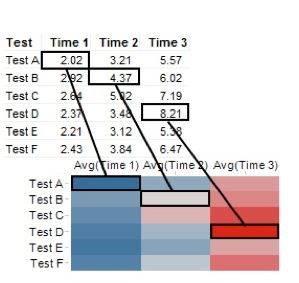
\includegraphics[scale=1]{Captura}
\caption{Heat map}
\label{fig:Captura}
\end{figure}

En la figura anterior se muestra un ejemplo de la técnica antes mencionada.\newline

Como base para nuestra investigación se tomo parte de lo que nos demuestra Blefari 
 \citep{Blefari} en donde nos muestra en codigo D3 un Simple heat map y nos permitió continuar con nuestra investigación para crear la visualización final.  
 
  \begin{figure}[h!]
\raggedright
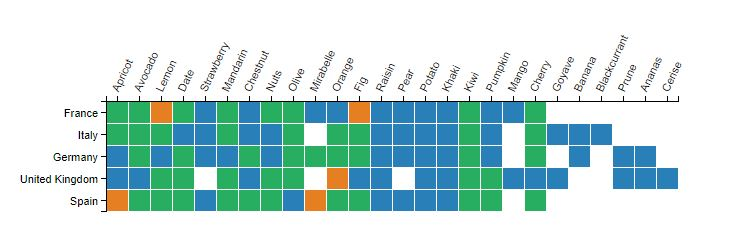
\includegraphics[scale=0.9]{Captura2}
\caption{Simple Heat map}
\label{fig:Captura 1}
\end{figure}

Además como última referencia de nuestra investigación, tomamos como ejemplo una técnica de visualización de barras por parte de Brush
\citep{Brush}
que nos permitió adaptar esta parte a nuestro proyecto.\newline

Además se utilizaron datos del Instituno Nacuional de Estadisticas y censos para las pruebas. 
\citep{INECNacimientos} 
\citep{INECAgropecuario}
\citep{INECMatrimonios}

\section{Implementación}

La estrategia utilizada para esta visualización se basó en la combinación de dos visualizaciones, el gráfico de barras y el "Heat Map".\\
Dicha implementación permite una visualización de datos más detallados de cada elemento mostrado en un Heat Map.\\
Esta implementación presenta deficiencias en cuanto el maping de los gráficos, ya que no son dinámicos, en su lugar se pensó en una versión mas sencilla de comprender (en cuanto código) donde la posición de las visualizaciones son fácilmente cambiadas por parámetros.
\newpage
El gráfico de barras puede contener cualquier cantidad de datos, y a su vez es dinámica en el tamaño de las barras mediante un algoritmo de mapeo que busca dividir el tamaño de las lineas en la cantidad de datos, y de ahí dibujarlas con un tamaño estándar.\\
Al ser interactivo, se notó que la manera más agradable de presentar ambos gráfico fue presentar el gráfico de barras de cada elemento del heat map cuando el cursor pasa encima de cada cuadro,esto permite una visualización fluida a cambio de utilización de mas recursos, cada gráfico de barras se hace y se mantiene mientras el cursor continúe encima del cuadro seleccionado.\\

\newpage

\section{Evaluación}

\begin{figure}[h!]
\centering
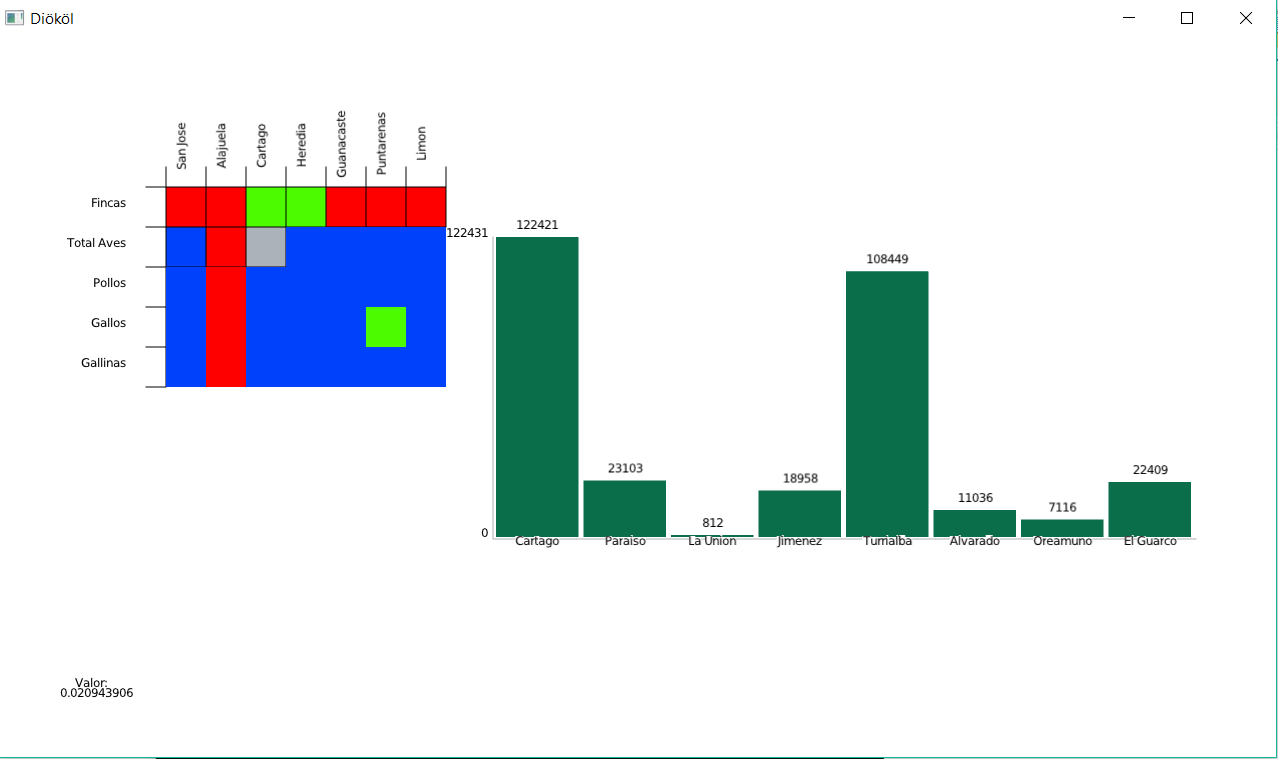
\includegraphics[scale=0.4]{1.png}
\caption{Gráfica de Total de fincas con aves de corral por cantidad de animales, 2014}
\label{fig:Captura 2}
\end{figure}


\begin{figure}[h!]
\centering
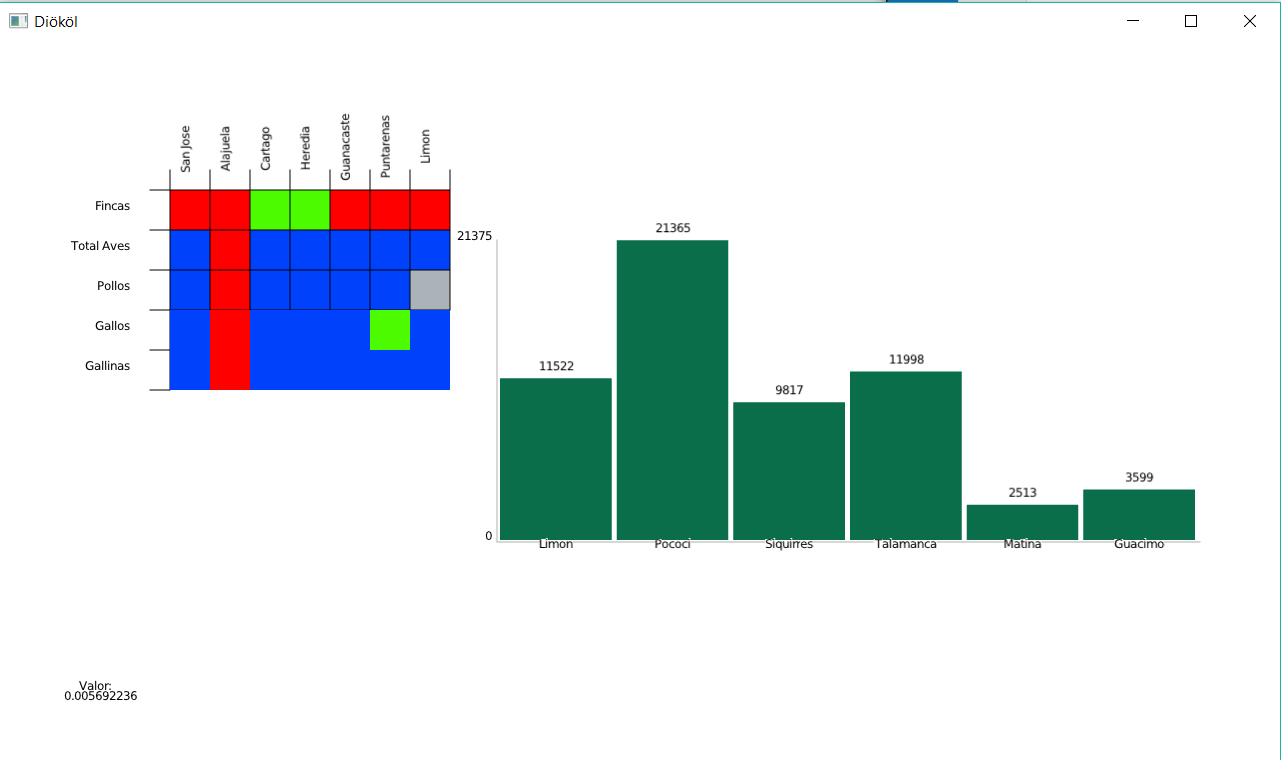
\includegraphics[scale=0.2]{2.png}
\caption{Gráfica de Total de fincas con aves de corral por cantidad de animales, 2014}
\label{fig:Captura 3}
\end{figure}


\begin{figure}[h!]
\centering
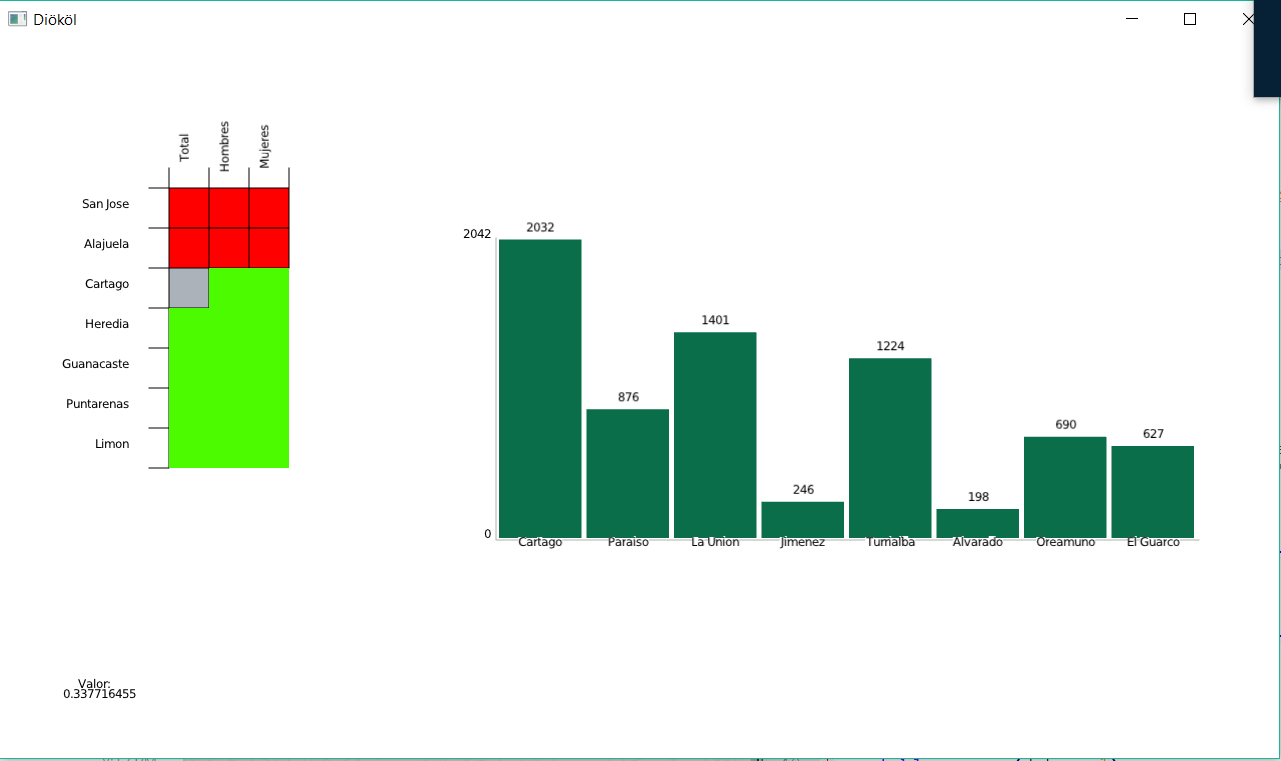
\includegraphics[scale=0.2]{3.png}
\caption{Total de matrimonios por grupos de edades, según sexo, condición de actividad y ocupación, 2017}
\label{fig:Captura 4}
\end{figure}


\begin{figure}[h!]
\centering
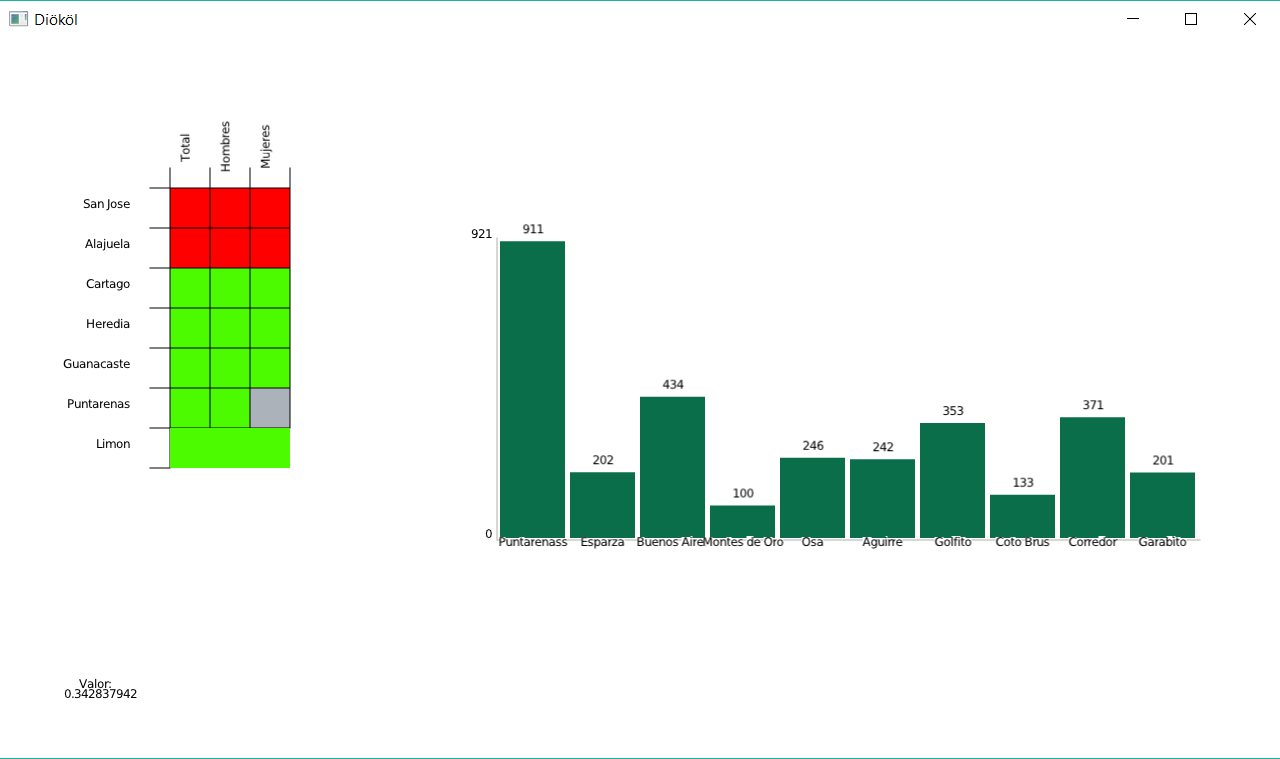
\includegraphics[scale=0.2]{4.png}
\caption{Total de matrimonios por grupos de edades, según sexo, condición de actividad y ocupación, 2017}
\label{fig:Captura 5}
\end{figure}


\begin{figure}[h!]
\centering
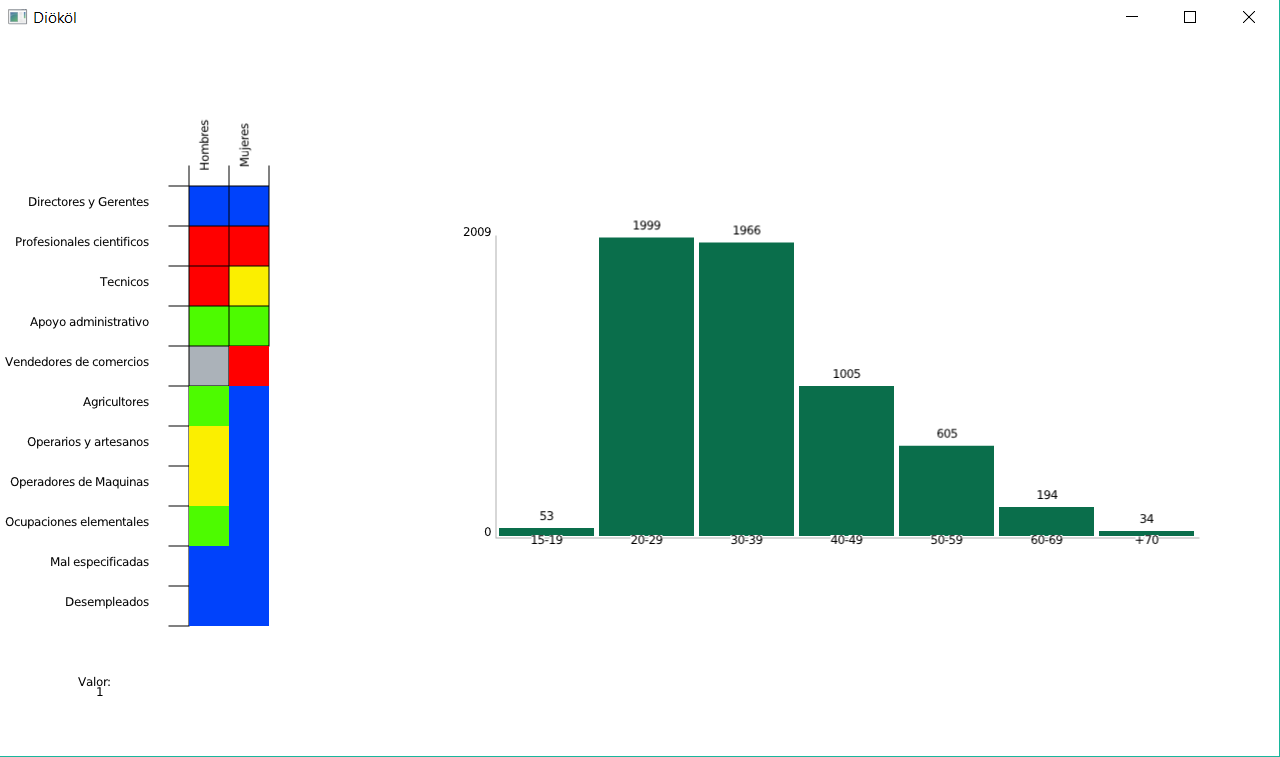
\includegraphics[scale=0.2]{5.png}
\caption{Total de nacimientos por sexo, según provincia y cantón de residencia de la madre, 2015}
\label{fig:Captura 6}
\end{figure}


\begin{figure}[h!]
\centering
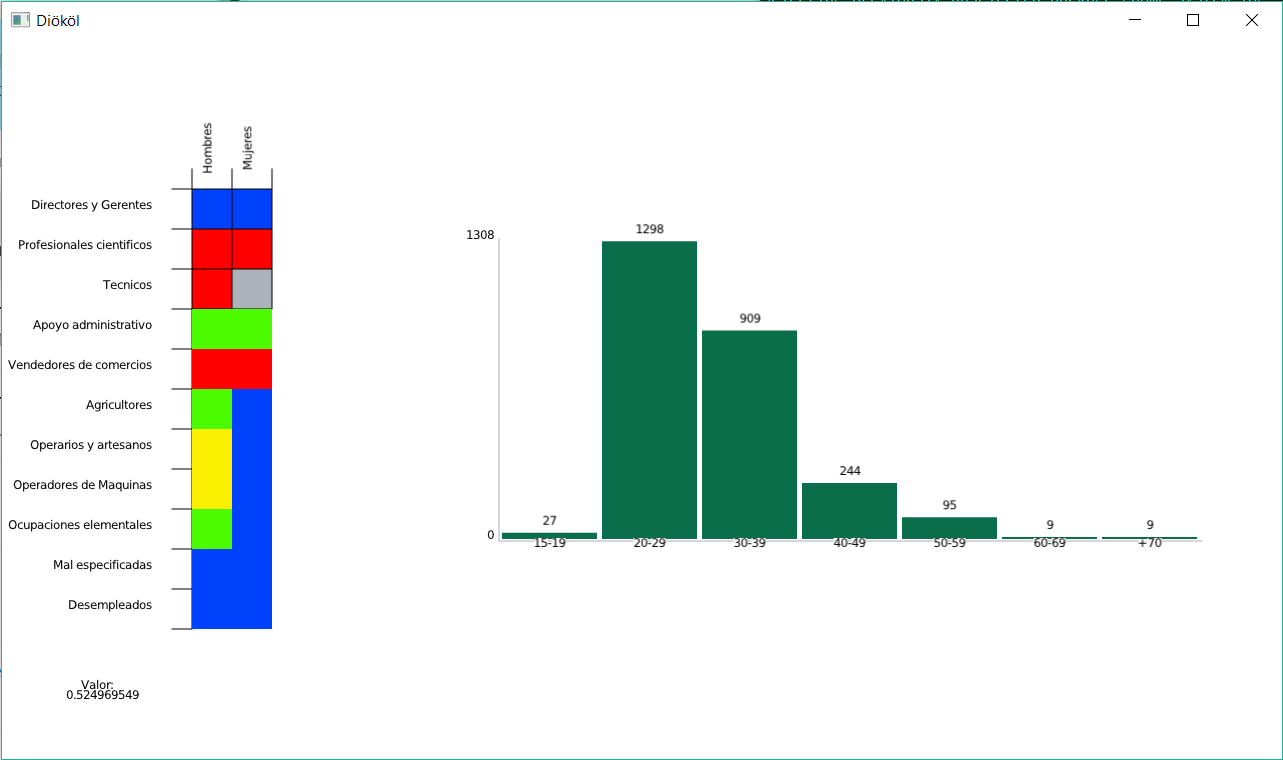
\includegraphics[scale=0.2]{6.png}
\caption{Total de nacimientos por sexo, según provincia y cantón de residencia de la madre, 2015}
\label{fig:Captura 7}
\end{figure}

\newpage
Los gráficos anteriores corresponden a grupos de datos descargados desde la página web del INEC. Los tres grupos de datos muestran como se puede representar una gran cantidad de datos de una forma más ordenada y limpia ocupando menos espacio. Lo anterior se logra mostrando gráficos de barras con información especifica, solamente cuando el usuario sitúa el mouse sobre alguno de los datos presentes en el heatmap.

\newpage

\section{Conclusión}

En conclusión se creó una visualización más agradable para presentar los datos, además se facilito la implementación en código de una manera significativa. Junto con las características agregadas a la visualización (que sea interactivo) y la capacidad de mantener grandes cantidades de datos hace a esta visualización una herramienta eficiente para visualizar datos de una manera cómoda y sencilla.

\bibliographystyle{plain}
\bibliography{references}
\end{document}
